\begin{table}
    \centering
    % 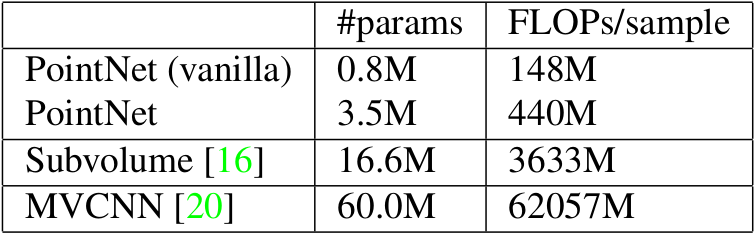
\includegraphics[width=0.4\textwidth]{complexity}
    \begin{tabular}{l|l|l}
        & \#params & FLOPs/sample \\ \hline
        PointNet (vanilla) & 0.8M & 148M \\
        PointNet & 3.5M & 440M \\ \hline
        Subvolume \cite{qi2016volumetric} & 16.6M & 3633M \\ \hline
        MVCNN \cite{su2015multi} & 60.0M & 62057M \\
    \end{tabular}
    \caption{
        \textbf{Time and space complexity of different deep learning
        architectures for 3D data classification.}
        PointNet (vanilla) is the classification PointNet without input and
        feature T-Net transformation networks. FLOP is floating-point
        operations. The ``M'' stands for a million units.
        Both Subvolume and MVCNN used input data pooling from multiple
        rotations or views, without which they have much inferior performance.
        % "\textbf{Time and space complexity of deep architectures for 3D data
        % classification.} PointNet (vanilla) is the classification PointNet
        % without input and feature transformations. FLOP stands for
        % floating-point operation. The “M” stands for million. Subvolume and
        % MVCNN used pooling on input data from multiple rotations or views,
        % without which they have much inferior performance."
        % Table and caption taken from \cite{qi2017pointnet}.
        % \todo{rewrite in own words}
        Table from \cite{qi2017pointnet}.
    } \label{table:complexity}
\end{table}
